\section{Auswertung}
\subsection{Bestimmung der maximalen Kraftflussdichte des verwendeten Aufbaus mit Magnetfeld}
Im Folgenden werden die Daten ausgewertet, die aufgenommen wurden, um das maximale Magnetfeld innerhalb des Aufbaus zu bestimmen. Wie bereits in Kapitel \ref{durchfuehrung} beschrieben, ist eine Messreihe mit einer Hall-Sonde durchgeführt worden; die erhaltenen Messwerte sind in Tabelle \ref{tab:messwerte_hall} zu sehen.
Graphisch aufgetragen sind ebendiese in Abbildung \ref{hall}. Zur Bestimmung des Maximums ist eine Ausgleichsrechnung der Form
\begin{equation}
B(z)=az^4+bz^3+cz^2+dz+e
\label{eq:regression}
\end{equation}
für die Messwerte $B(z)>100$ durchgeführt worden.
Als Regressionsparameter ergeben sich
\begin{align*}
  a&=-\SI{0,0076 \pm 0,0007}{mTmm^{-4}}\\
  b&=\SI{0,39 \pm 0,06}{mTmm^{-3}}\\
  c&=-\SI{7,6 \pm 0,7}{mTmm^{-2}}\\
  d&=\SI{6,6 \pm 6,0}{mTmm^{-1}}\\
  e&=-\SI{215 \pm 2}{mT}.
\end{align*}
Über die Ableitung der Regressionsfunktion \eqref{eq:regression}
\begin{equation}
\frac{\text{d}}{\text{dz}}B(z)=4a^3+3b^2+2c+d \stackrel{!}{=} 0
\end{equation}
und dem Umstellen nach $z$ folgt ein Maximalwert von
\begin{equation}
 z_\text{max}=\SI{128,24}{mm}.
\end{equation}
Hierüber folgt durch Einsetzen in Formel \eqref{eq:regression}
\begin{equation}
B_\text{max}=\SI{414,5}{mT}.
\end{equation}
\begin{table}[h]
  \footnotesize
  \centering
  \caption{Mit einer Hall-Sonde gemessene Magnetfeldstärke im Bereich des Luftspalts zur Bestimmung des Maximalwerts.}
  \label{tab:messwerte_hall}
  \begin{tabular}{S[table-format=1.1] S S}
    {$z$ / mm} & {$B$ / mT}\\
    \midrule
    100 & 0 \\
    105 & 3 \\
    110 & 14\\
    111 & 20 \\
    112 & 27 \\
    113 & 35 \\
    114 & 48 \\
    115 & 68 \\
    116 & 95 \\
    117 & 135 \\
    118 & 183 \\
    119 & 241 \\
    120 & 304 \\
    121 & 341 \\
    122 & 368 \\
    123 & 382 \\
    124 & 393 \\
    125 & 402 \\
    126 & 407 \\
    127 & 409 \\
    128 & 411 \\
    129 & 410 \\
    130 & 408 \\
    131 & 408 \\
    132 & 404 \\
    133 & 399 \\
    134 & 390 \\
    135 & 378 \\
    136 & 364 \\
    137 & 335 \\
    138 & 308 \\
    139 & 263 \\
    140 & 207 \\
    141 & 163 \\
    142 & 106 \\
    143 & 77 \\
    144 & 54 \\
    145 & 39 \\
    146 & 30 \\
    147 & 21 \\
    148 & 16 \\
    149 & 12 \\
    150 & 8 \\
    151 & 6 \\
    152 & 5 \\
    153 & 3 \\
    154 & 2 \\
    155 & 2 \\
    160 & 0 \\
  \end{tabular}
\end{table}
\clearpage
\begin{figure}[H]
  \centering
  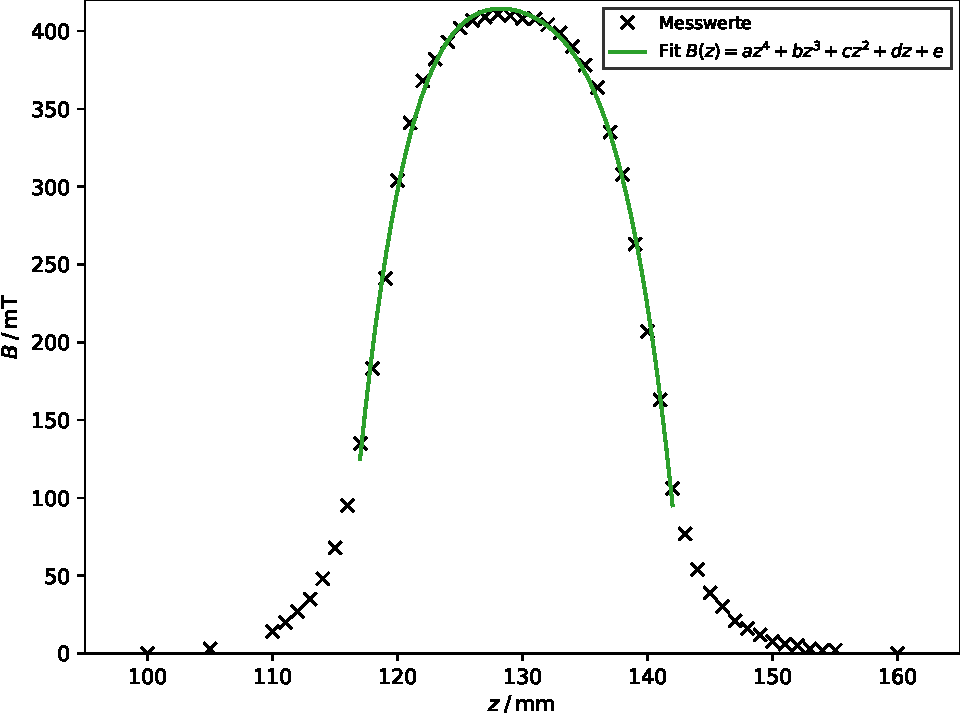
\includegraphics[width=0.8\textwidth]{plots/hall.pdf}
  \caption{Die magnetische Kraftflussdichte $B$ aufgetragen gegen die Längenkoordinate $z$ innerhalb der Magnetspulen. Zur Bestimmung des Maximalwertes von $B$ ist eine Ausgleichsrechnung der Form $B(z)=az^4+bz^3+cz^2+dz+e$ eingezeichnet.}
  \label{hall}
\end{figure}

\subsection{Bestimmung der effektiven Masse}
Für die Faraday-Rotation wird Licht im Wellenlängenbereich von $\SI{1,06}{µm}$ und $\SI{2,65}{µm}$ verwendet.
Die durch Filtern erzeugten neun Wellenlängen sind in den Tabellen \ref{tab:probe1}, \ref{tab:probe2} und \ref{tab:probe3} zu sehen.
Es folgt die Auswertung der drei Proben mit den Parametern
\begin{align*}
d_\text{hochrein}&=\SI{5,11}{mm}\\
d_{N=1,2\cdot10^{18}}&=\SI{1,36}{mm}\\
d_{N=2,58\cdot10^{18}}&=\SI{1,296}{mm}.
\end{align*}
Hierbei ist die erste benannte Probe $d_\text{hochrein}$ die hochreine und die beiden letzten die dotierten $\ce{GaAs}$-Proben mit der Dotierkonzentration $N$.\\
Es werden die Differenzen der beiden abgelesenen Winkel zu
\begin{equation}
  \theta=\theta_1-\theta_2
\end{equation}
bestimmt. Diese Winkelgrößen und die daraus abgeleitete Größe $\theta/d$ sind in den Tabellen \ref{tab:probe1}, \ref{tab:probe2} und \ref{tab:probe3} eingetragen.
In der Abbildung \ref{GaAs1} wird $\theta/d$ gegen $\lambda^2$ aufgetragen.\\
Darüber hinaus wird die Differenz der normierten Rotationswinkel $\theta/d$ der beiden dotierten $\ce{GaAs}$-Proben mit den Daten der hochreinen Probe in Abbildung \ref{GaAs2} gebildet und dargestellt.
Für das Ermitteln der effektiven Massen werden zwei lineare Ausgleichsrechnungen der Form
\begin{equation}
  f(\lambda^2)=\theta/d(\lambda^2)=a\lambda^2+b
\end{equation}
erstellt, aus denen sich die folgenden Parameter ergeben:
\begin{align*}
&\text{hochreine Probe - n-dotiert}\; N=\SI{1.2e18}{\centi\meter^{-3}}:\\
&a_1=-\SI{16,0 \pm 12,9}{\meter^{-3}}\\
&b_1=\SI{90,99 \pm 56,33}{\meter^{-1}}\\
&\text{hochreine Probe - n-dotiert}\; N=\SI{2.8e18}{\centi\meter^{-3}}:\\
&a_2=\SI{4,1\pm29,7}{\meter^{-3}}\\
&b_2=\SI{121,5\pm129,9}{\meter^{-1}}
\end{align*}

Für das Bestimmen der effektiven Massen wird Gleichung \ref{eq:theta2} nach der gesuchten Größe umgestellt, sodass sich
\begin{equation}
m^{*} = \sqrt{\frac{e_0^3}{8\pii^2 \varepsilon_0 c^3} \frac{N B_\text{max}}{n} \frac{1}{a}}
\end{equation}
als Zusammenhang ergibt. Werden nun die Regressionsparameter $a_1$ und $a_2$ aus dem vorherigen Schritt benutzt, so ergeben sich
\begin{align*}
  m_1^{*} &= -\\
  \shortintertext{für die $\ce{GaAs}$-Probe mit $N=\SI{1.2e18}{\centi\meter^{-3}}$ und}
  m_2^{*} &= (\num{1 \pm 5e2})m_\text{e}
\end{align*}
für die $\ce{GaAs}$-Probe mit $N=\SI{2.8e18}{\centi\meter^{-3}}$, in Einheiten der Ruhemasse $m_\text{e}$ der Elektronen.
Aufgrund der negativen Steigung bei der ersten Probe, lässt sich keine effektive Masse bestimmen.
Der benötigte Brechungsindex für Galliumarsenid von $n=3,3543$ ist der Literatur entnommen worden \cite{Brechungsindex}.
Es liegt eine Abweichung zu dem bestimmten Theoriewert der effektiven Masse $m^{*}=0,067m_\text{e}$ \cite{effmasse} von $\SI{149253}{\%}$ vor.
\begin{table}[h]
  \centering
  \caption{Messwerte und die daraus abgeleiteten Größen $\Theta$ und $\Theta/d$ der Messung zur n-dotierten $\ce{GaAs}$-Probe mit $N=\SI{1.2e18}{\centi\meter^{-3}}$.}
  \label{tab:probe1}
  \begin{tabular}{S[table-format=1.1] S S S S}
    {$\lambda$ / µm} & {$\theta_1$ / °} & {$\theta_2$ / °} & {$\theta$ / rad} & {$\frac{\theta}{d}$ / rad $m^{-1}$}\\
    \midrule
    1,06 &  168,05 &  158,00 & 0.1754 & 128,97\\
    1,29 &  210,92 &  196,00 & 0.2604 & 191,47\\
    1,45 &  205,92 &  200,75 & 0.0902 & 66,32\\
    1,72 &  161,20 &  158,00 & 0.0558 & 41.03\\
    1,96 &  165,20 &  146,50 & 0.3263 & 239,93\\
    2,156 & 166,20 &  161,00 & 0.0907 & 66,69\\
    2,34 & 200,40 &  187,00 & 0.2338 & 171,91\\
    2,51 & 255,00 &  250,75 & 0.0741 & 54,49\\
    2,65 & 299,00 &  294,00 & 0.0872 & 64,12\\
  \end{tabular}
\end{table}

\begin{table}[h]
  \centering
  \caption{Messwerte und die daraus abgeleiteten Größen $\Theta$ und $\Theta/d$ der Messung zur n-dotierten $\ce{GaAs}$-Probe mit $N=\SI{2,8e18}{\centi\meter^{-3}}$.}
  \label{tab:probe2}
  \begin{tabular}{S[table-format=1.1] S S S S}
    {$\lambda$ / µm} & {$\theta_1$ / °} & {$\theta_2$ / °} & {$\theta$ / rad} & {$\frac{\theta}{d}$ / rad $m^{-1}$}\\
    \midrule
    1,06 &  279,48 &  275,58 & 0.0680 & 52,47\\
    1,29 &  234,25 &  207,08 & 0.4742 & 348,68\\
    1,45 &  256,50 &  245,15 & 0.1980 & 145,59\\
    1,72 &  296,62 &  270,36 & 0.4583 & 336,99\\
    1,96 &  280,33 &  269,33 & 0.1919 & 141,10\\
    2,156 & 275,35 &  267,03 & 0.1452 & 106,76\\
    2,34 & 307,82 &  290,43 & 0.3035 & 223,16\\
    2,51 & 292,66 &  262,00 & 0.5351 & 393,46\\
    2,65 & 295,05 &  282,05 & 0.2268 & 166,76\\
  \end{tabular}
\end{table}

\begin{table}[h]
  \centering
  \caption{Messwerte und die daraus abgeleiteten Größen $\Theta$ und $\Theta/d$ der Messung zur hochreinen Probe.}
  \label{tab:probe3}
  \begin{tabular}{S[table-format=1.1] S S S S}
    {$\lambda$ / µm} & {$\theta_1$ / °} & {$\theta_2$ / °} & {$\theta$ / rad} & {$\frac{\theta}{d}$ / rad $m^{-1}$}\\
    \midrule
    1,06 &  243,00 &  226,78 & 0.2830 & 55,38\\
    1,29 &  259,82 &  240,07 & 0.3447 & 67,46\\
    1,45 &  241,25 &  221,62 & 0.3426 & 67,05\\
    1,72 &  175,25 &  166,02 & 0.1610 & 31,51\\
    1,96 &  262,12 &  181,33 & 1.4100 & 275,93\\
    2,156 & 178,28 &  171,23 & 0.1230 & 24,07\\
    2,34 & 184,42 &  178,50 & 0.1033 & 20,22\\
    2,51 & 188,42 &  168,33 & 0.3506 & 68,61\\
    2,65 & 203,65 &  156,15 & 0.8290 & 162,23\\
  \end{tabular}
\end{table}
\clearpage
\begin{figure}[H]
  \centering
  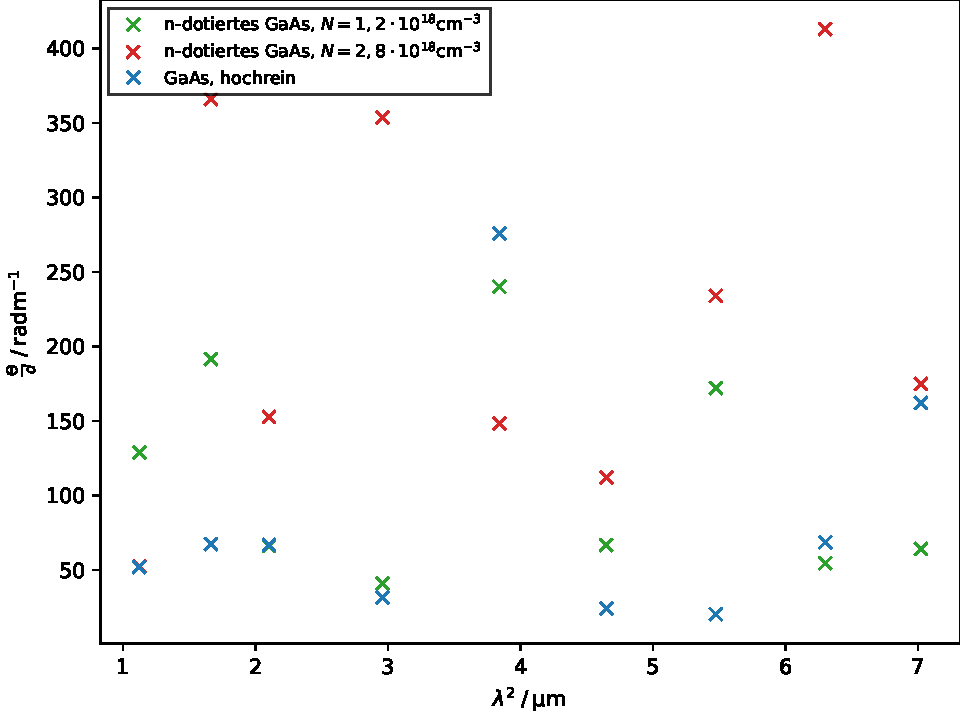
\includegraphics[width=0.8\textwidth]{plots/GaAs.pdf}
  \caption{Die normierte Faraday-Rotation $\theta/d$ aufgetragen gegen das Quadrat der Wellenlänge $\lambda$ für die n-dotierten und die hochreine $\ce{GaAs}$-Probe.}
  \label{GaAs1}
\end{figure}

\begin{figure}[H]
  \centering
  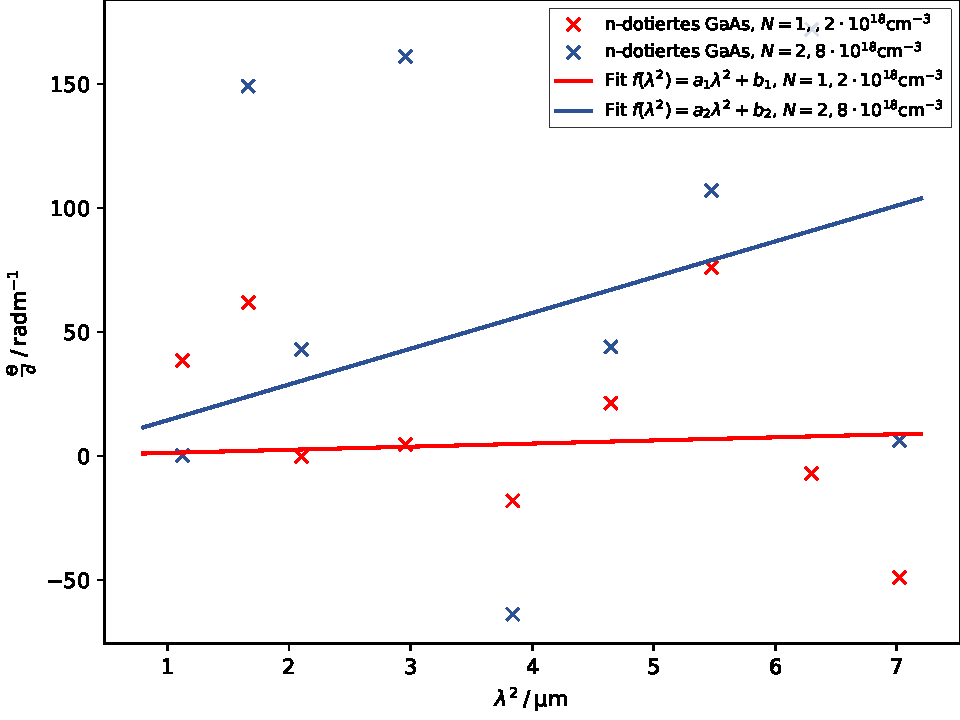
\includegraphics[width=0.8\textwidth]{plots/GaAs2.pdf}
  \caption{Die Differenz der normierten Faraday-Rotationen der dotierten $\ce{GaAs}$-Proben mit denen der hochreinen $\ce{GaAs}$-Probe aufgetragen gegen $\lambda^2$.}
  \label{GaAs2}
\end{figure}
\clearpage
